\documentclass[a4paper,11pt]{article}

\usepackage{mlassn}
%\excludecomment{solution}

\begin{document}

\makeheader{2}                              					% assignment number
           {September 19, 2017}      			           		% assignment date
					 {100}																				% total marks

\begin{mlproblem}[Oh holy ID3, show me how to grow a tree!]{2+3+10+0=15}
Consider the following toy dataset that you can use to learn how to choose an advisor.
\begin{table}[h!]
\centering
{\small
\begin{tabular}{| c | l | c | c | c | c | c |}
	\hline
	S.No. & Name  & $\substack{\text{Size of}\\\text{research group}}$ & $\substack{\text{Like the}\\\text{research area?}}$ & $\substack{\text{Average}\\\text{workload?}}$ & $\substack{\text{\# of meetings}\\\text{per week}}$ & $\substack{\text{Good}\\\text{advisor}}$? \\ \hline
	1 & Prof. R. Lupin & small  & yes & average  & $2-3$ & no \\ \hline
	2 & Prof. P. Sprout & large  & no  & average  & $0-1$ & yes \\ \hline
	3 & Prof. R. Hagrid & small  & no  & average  & $> 3$ & no \\ \hline
	4 & Prof. C. Binns & medium & no  & heavy & $0-1$ & no \\ \hline
	5 & Prof. A. Sinistra & large  & no  & heavy & $0-1$ & no \\ \hline
	6 & Prof. S. Snape & medium & no  & heavy & $0-1$ & yes \\ \hline
	7 & Prof. S. Kettleburn & small  & no  & light & $> 3$ & no \\ \hline
	8 & Prof. Firenze & small  & no  & average  & $2-3$ & no \\ \hline
	9 & Prof. S. Vector & small  & yes & average  & $0-1$ & yes \\ \hline
	10 & Prof. R. Hooch & medium & no  & light & $0-1$ & no \\ \hline
	11 & Prof. C. Burbage & large  & no  & average  & $0-1$ & yes \\ \hline
	12 & Prof. A. P. W. B. Dumbledore & medium & yes & light & $0-1$ & yes \\ \hline
	13 & Prof. S. Trelawney & small  & no  & light & $2-3$ & no \\ \hline
	14 & Prof. H. Slughorn & medium & no  & heavy & $0-1$ & no \\ \hline
	15 & Prof. Q. Quirrell & large  & yes & heavy & $0-1$ & no \\ \hline
\end{tabular}
}
\end{table}

\begin{enumerate}
	\item Is the first attribute (name) useful in learning a binary classifier from this data? Why?
	\item Is it possible to perfectly classify this data (no matter how complicated the classification algorithm)? Why?
	\item Read about the ID3 decision tree learning algorithm. There are many nice resources available for this online. The following website does a nice job with examples \url{https://www.cise.ufl.edu/~ddd/cap6635/Fall-97/Short-papers/2.htm}. Build a decision tree using the ID3 algorithm on the data given above. You may stop splitting nodes that are at depth 2 or more (the root of the tree is depth 0). For any impure leaves, use the majority label at that leaf to take a decision for data points in that leaf. Break any ties arbitrarily.
	\item \emph{Fake Bonus}: Can you guess which research areas do I like?
\end{enumerate}

\begin{figure}[h!]%
\centering
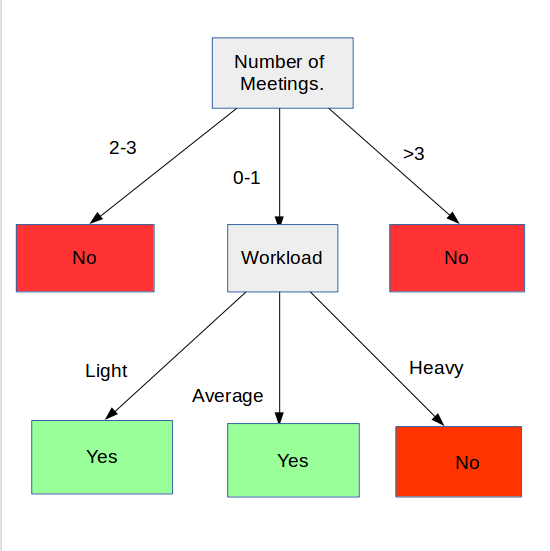
\includegraphics[width=0.75\columnwidth]{dt.png}%
\caption{A sample decision tree -- not necessarily the one that ID3 would generate :).}%
\end{figure}

Draw the decision tree that you have learnt (see sample above) and include it in your PDF file as an image. You do not need to write/submit code for this problem. However, you do need to justify the following:
\begin{enumerate}
	\item Why you chose to split a certain node along such and such attribute. Do this by giving numerical values of the information gain corresponding to various attributes at various nodes as you calculated them. Just give the final values -- no calculations need be shown.
	\item Why you chose not to split certain nodes further and make them a leaf.
\end{enumerate}
\emph{Statutory Warning}: Don't use this tree to select an advisor in real life.
\end{mlproblem}

\begin{mlproblem}[Guess my Grocery List]{5+5+10=20+bonus}
I run a supermarket called ML-mart that stores $L$ items. The $j\nth$ item has cost $c_j \in \bR$. The $i\nth$ customer in ML-mart is represented as a $d$-dimensional real vector $\vx^i$. Customer $i$ always buys the same subset of items $S^i \subset [L]$ and pays the bill $b^i = \sum_{j \in S^i}c_j + \epsilon^i$ where $\epsilon^i \sim \cN(0,\sigma^2)$ (where $\sigma$ is the same for all users but not known to you) is some noise in the bill amount. The noise is to account for the fact that maybe the person bought some items, say \emph{mirchi} and \emph{dhaniya} -- chillies and cilantro, which are not in the list of $L$ items, in addition to items in the set $S^i$ or else had a coupon for a small discount.

However, something went wrong with my billing machine and it erased all records of which of the $L$ items did the customer buy! The only thing the billing machine stored was the customer ID $\vx \in \bR^d$ and the bill that customer paid $b \in \bR$. I have such incomplete records for $n$ customers $(\vx^i,b^i)_{i=1,\ldots,n}$. Can you help me complete my bills by figuring out which items the customers bought? 

\begin{enumerate}
	\item Cast the above problem as a latent variable learning problem and develop a sound generative story for the same
	\item Write down the complete likelihood expression for the observed data
	\item Design a hard-assignment alternating optimization algorithm to solve the problem
	\item \emph{Bonus 1}: Design a soft-assignment alternating optimization algorithm for the problem
	\item \emph{Bonus 2}: Can you design a hard-assignment alternating optimization algorithm that works in $\bigO{ndL}$ time? It seems the problem reduces to the problem of finding the largest sum principal matrix of an $L \times L$ matrix (that is a sum of a rank-1 matrix and a diagonal matrix) for which I could neither find any NP-hardness result nor any polytime algorithm. Do let me know if you have any idea.
\end{enumerate}

You may assume that $d,n,L$ are not very large (say $L \approx 10$, $d \approx 100$, $n \approx 1000$) and you do not need to worry about the challenges of the kind we encountered in large-scale multi-label learning (as we discussed in lecture 6). Your solution may use upto $\bigO{2^L\cdot n\cdot d}$ time and memory without any hesitation (notice the $2^L$). To get you started, here are a few tips
\begin{enumerate}
	\item Your model $\vTheta$ need not be generative, i.e. it is not necessary to model $\P{b,\vx\cond\vTheta}$. You can be discriminative, i.e. just model $\P{b\cond\vx,\vTheta}$.
	\item Use a linear logistic model conditioned on user features $\vx^i$ to account for users selecting items (see lecture 6).
	\item Assume that items are bought independently i.e. for any user $i$ and any model $\vTheta$, we have $\P{(j_1,j_2) \in S^i \cond \vx^i,\vTheta} = \P{j_1 \in S^i \cond \vx^i,\vTheta}\cdot\P{j_2 \in S^i \cond \vx^i,\vTheta}$. This may remind you of the the naive Bayes assumption and will play a similar simplifying role here.
	\item However, be careful. If you are conditioning on $b^i$, e.g., looking at $\P{(j_1,j_2) \in S^i \cond \vx^i,b^i,\vTheta}$, then the items can no longer be assumed to have been independently bought since the price one has paid restricts which items could be bought together (e.g. if $b^i$ is small then the customer could not have purchased many expensive items together).
	\item For elementary problems for which we have already seen solutions in class, you need not explain how to solve them. For example, if your proposed algorithm requires you to solve a few ridge regression/SVM problems, just say that such and such technique from lecture number so and so can be used to solve the ridge regression/SVM problem. However, please use this freedom sensibly -- please don't use it to just point to the soft assignment lecture and end your solution there :)
	\item Do not worry about whether your algorithm will converge, will it converge to a local minima or a saddle point etc. You are solving an NP-hard problem here. Just develop a sensible algorithm for now.
\end{enumerate}
\end{mlproblem}

\begin{mlproblem}[The Daft Dual]{10+2+10+3=25+bonus}
Consider the following problem formulation for $n$ binary labelled data points $(\vx^i,y^i)_{i=1,\ldots,n}$ where $\vx^i \in \bR^d$ and $y^i \in \bc{-1,+1}$
\begin{align*}
\underset{\vw,\bc{\xi_i}}{\arg\min}&\ \norm{\vw}_2^2 + \sum_{i=1}^n\xi_i^2\\
\text{s.t.} &\ y^i\ip{\vw}{\vx^i} \geq 1 - \xi_i, \text{ for all } i \in [n] \qquad\qquad{(P1)}\\
&\ \xi_i \geq 0, \text{ for all } i \in [n]
\end{align*}
This is a variant of the SVM formulation. Using a technique similar to the one you used for the ``Break Free from Constraints'' problem in Assignment 1, you can show that $(P1)$ is equivalent to minimizing the regularized squared hinge loss (see lecture 7). However, this question is not about that. We are more interested in solving this optimization problem now.
\begin{enumerate}
	\item Show that the constraints $\xi_i \geq 0$ are vacuous i.e. the optimization problem does not change even if we remove the all constraints $\xi_i \geq 0$ for all $i \in [n]$.
	\item Write the Lagrangian for $(P1)$.
	\item Give the derivation for the Lagrangian dual problem for $(P1)$.
	\item What are the differences between the dual problem for $(P1)$ and the dual problem for the original SVM problem? The dual for the original SVM problem may be referred to, for example, in [\textbf{DAU}] equation 11.38.
	\item \emph{Bonus}: Are the positivity constraints $\xi_i \geq 0$ vacuous for the original SVM problem as well? Recall that the original SVM has the term $\sum_{i=1}^n\xi_i$ in its objective instead of $\sum_{i=1}^n\xi_i^2$. Why can/cannot we remove the positivity constraints from the original SVM problem without changing the solution?
\end{enumerate}
It is advisable that you become comfortable with the derivation of the dual of the original SVM problem with slack variables (see [\textbf{DAU}] S. 7.7 S. 11.5-11.6, [\textbf{SSBD}] S. 15.3-15.5) before attempting this problem. Note that in the lecture, we only looked at a simplified version of the SVM problem without slack variables.
\end{mlproblem}

\begin{mlproblem}[My First SVM Solver]{40}
In this problem we will design a primal and a dual solver for the SVM problem. We have with us a data set with $n$ data points each with a $d$ dimensional feature vector and a binary label $(\vx^i,y^i)$, with $\vx^i \in \bR^d$ and $y^i \in \bc{-1,+1}$. On this dataset we wish to minimize the following function 
\[
\min_{\vw \in \bR^d} f(\vw),
\]
where
\begin{align*}
f(\vw) = \frac{1}{2}\norm{\vw}_2^2 + \sum_{i=1}^n\bs{1 - y^i\ip{\vw}{\vx^i}}_+
\end{align*}

The Lagrange dual of this problem is the following
\begin{align*}
\min_{\valpha \in \bR^n}&\ \frac{1}{2} \valpha^\top Q \valpha - \sum_{i=1}^n\valpha_i\\
\text{s.t.}&\ 0 \leq \valpha_i \leq 1, \text{ for all } i \in [n],
\end{align*}

where $Q \in \bR^{n \times n}$ with $Q_{ij} = y^iy^j\ip{\vx^i}{\vx^j}$. If we find an $\hat\valpha$ that is (near)-optimal, we can use it to reconstruct a model vector as $\hat\vw = \sum_{i=1}^n\valpha_iy^i\vx^i$. You have been supplied with a training data set with 300K data points, each point being 54 dimensional. This is a supervised binary classification problem. However, each feature vector is very sparse. Only around 11-12 of the 54 dimensions are non-zero in any data point. Download this dataset from the URL

{\small \url{http://web.cse.iitk.ac.in/users/purushot/courses/ml/2017-18-a/material/assn2data.zip}}\\

Your job is to design two SVM solvers to minimize the function $f(\vw)$ over the entire training set. You may use the training data provided to you in any way to tune your parameters (e.g. step length) by splitting into validation sets in any fashion (e.g. held out, k-fold). You are also free to use any fraction of the training data for validation, etc. but your job is to do well in terms of minimizing the objective function $f(\vw)$ on the training set (as well as a secret test set which we have with us and will not reveal to you). Execute the following
\begin{enumerate}
	\item (Part I) Write a solver to execute the gradient descent (GD) algorithm on the primal problem to minimize $f(w)$ (not SGD, not coordinate descent but vanilla gradient descent).
	\item (Part II) Write a solver to execute the stochastic coordinate descent (SCD) algorithm (lec10.pdf page 63) on the dual problem. Since the dual problem has a constraint, you will have to use a projection step.
	\item (Part III) For the GD solver, does the current iterate $\vw^t$ give better performance or the averaged iterate $\bar{\vw}^t = \frac{1}{t}\sum_{\tau=1}^t\vw^\tau$ (See [\textbf{SSBD}] section 14.3 and Piazza discussion \url{https://piazza.com/class/j5toxxryhdx56k?cid=276}). The averaging trick works for SGD but is helpful for GD as well when the function being optimized is non-differentiable. Averaging is not required for SCD since the objective function in the dual is smooth and differentiable.
	\item (Part IV) What step length selection strategy worked best for GD?
	\item (Part V) On the same graph, with time elapsed (the variable \verb|time_elapsed| in the skeleton code) till now on the x-axis and objective value $f(\vw)$ (over the entire training set of 300K points) on the y-axis, plot the progress of the GD and SCD algorithms for a comparison. The skeleton code stops the SCD/GD procedure after every few iterations to take the current model $\vw^t$ (or the current averaged model $\bar{\vw}^t$ if you find that more helpful) and evaluate $f(\vw^t)$. Does GD reduce the objective value $f(\vw)$ faster or does SCD reduce the objective value $f(\vw)$ faster?
	\item (Part VI) There are two ways of measuring time spent -- one is wall-clock time (the variable \verb|time_elapsed| in the skeleton) and the other is theoretical time (number of iterations till now * amount of work done for each iteration) where
	\begin{enumerate}
		\item number of iterations till now = \verb|tick_vals|* \verb|spacing|
		\item amount of work per iteration is $nd$ for GD and $d$ for SCD
	\end{enumerate}
	Plot the above graphs again using theoretial time on the x-axis. Do you see a difference? Please note that in both set of graphs there will be \verb|n_iter|/\verb|spacing| points on the graph (see the skeleton code).
\end{enumerate}

You are highly encouraged to read the following paper from ICML 2008 \url{http://www.csie.ntu.edu.tw/~cjlin/papers/cddual.pdf} and use equation (9) while building the solver for Part II. Using equation (9) from the paper will allow you to minimize the objective completely along a coordinate instead of taking just a gradient step. Students using this more advanced step are bound to get much faster solvers than those that implement the mediocre projected stochastic coordinate descent algorithm.

Some points of advice regarding the implementation are given below. There are skeleton files \verb|solver_GD.py| and \verb|solver_SCD.py| included in the assignment package. Do look at them.

\begin{enumerate}
	\item In the notation of the paper, we will use $D_{ii} = 0$ and $U = 1$ in equation (9).
	\item You do not have to implement the ``shrinking'' step proposed in the ICML 2008 paper.
	\item Choose a random coordinate to minimize at each step for Part II. The ICML 2008 paper uses a more involved strategy which you need not implement.
	\item Do remember that if implemented naively, coordinate descent can take $\bigO{nd}$ time at each step. You will have to do careful bookkeeping (see for example lec10.pdf page 90) to make sure each step takes only $\bigO{d}$ time or so.
	\item Remember that the data points you have been given are very sparse. The skeleton file will load the data into a compressed sparse row (CSR) matrix. You may choose to densify the matrix or else keep it sparse. Keeping it sparse will yield speedups.
	\item You do not require Shogun for this assignment.
	\item You are not allowed to use any sklearn, scipy, pandas etc library functions. The only functions you are allowed to use have already been inserted into the skeleton file.
\end{enumerate}

\end{mlproblem}

\end{document}